% Template for ICIP-2022 paper; to be used with:
%          spconf.sty  - ICASSP/ICIP LaTeX style file, and
%          IEEEbib.bst - IEEE bibliography style file.
% --------------------------------------------------------------------------
\documentclass{article}
\usepackage{algorithm,algpseudocode,bm,cancel,spconf,amsmath,amssymb,graphicx,verbatim}

\title{Maximum Likelihood Multiframe Registration Under Constant Translation}
\name{Evan Widloski and Farzad Kamalabadi}
\address{University of Illinois Urbana-Champaign}

% ------------------- Macros ----------------------
% probability equals sign
\newcommand\peq{\mkern1.5mu{=}\mkern1.5mu}
% likelihood center pipe
\newcommand\lpipe{\mkern1.5mu{|}\mkern1.5mu}
% correlation
\newcommand\lstar{\mkern4mu{\star}\mkern4mu}

% ------------------- Header ----------------------
\begin{document}
\maketitle
\begin{abstract}
  We present a registration algorithm which jointly estimates motion and the ground truth image from a set of noisy frames under rigid, constant, translation.  With additive white Gaussian noise, the algorithm is optimal in the maximum likelihood sense.  Furthermore, the algorithm is non-iterative and has no hand-tuned parameters, requiring a fixed number of FFT, multiplication, and downsampling operations which are commonly available on embedded imaging systems.  The accuracy is compared to other algorithms of the same class.  Our algorithm outperforms other pairwise or multiframe methods without an explicit motion model, especially in the low SNR regime.
\end{abstract}

\begin{keywords}
  registration, maximum likelihood, low SNR, motion estimation, embedded signal processing
\end{keywords}

% ------------------- Introduction ----------------------
\section{Introduction}
\label{sec:introduction}

Image alignment, or image registration is a classic problem in the field of image processing in which an image or image sequence must be aligned after some unknown spatial transformation.
Registration is an important preprocessing step in image processing pipelines involving change detection, image mosaicing, and super-resolution with applications in medical imaging \cite{wells1996multi}, computer vision tasks \cite{mers}, military surveillance \cite{konrad}, and remote-sensing.

A wide range of techniques have been developed over the preceding decades, with varying models on the type of motion allowed between frames, content of the scene, changes to objects within the scene, and computational resources available.  In particular we have developed a progressive \cite{robinson2004fundamental}, area-based \cite{zitova2003image} \cite{brown1992survey} registration algorithm derived from an explicit noise model and shown to be optimal in maximum likelihood (ML).

There have been several publications which propose an ML approach to registration, starting with Bradley \cite{bradley1973equivalence}, who showed an equivalence between ML and least squares estimates along with Kumar \cite{kumar1992correlation} specifically for registration under additive white Gaussian noise (AWGN).  Later, Mort \& Srinath \cite{mort1988maximum} developed an ML subpixel registration algorithm for pairs of Nyquist-sampled images.  Guillaume, et al. \cite{guillaume1998maximum} and Gratadour et al. \cite{gratadour2005sub} developed a method for a sequence of low SNR astronomical image frames under Poisson and Gaussian noise, which was minimized iteratively.  Guizar-Sicairos, Thurman \& Fienup \cite{guizar2008efficient} proposed an efficient subpixel scheme by upsampling in the frequency domain with direct DFT evaluations.

Our algorithm is motivated by astronomical imaging, where long integration times are sometimes necessary to have sufficient SNR in low light caused by target faintness or low optical efficiency of the imaging system.  However, longer integration times can induce significant motion blur in the images being captured, reducing angular resolution.  Instead, if shorter integration times in a sequence of images can be fused, longer effective integration time can be attained without the associated increase in motion blur.

In particular, our algorithm was conceived for the upcoming VISORS mission, a formation flying cubesat mission studying the solar corona at high resolution \cite{gundamraj2021preliminary}, where the motion of the scene is approximately constant translation throughout the 10 second capture window.  This stronger assumption about the motion allows us to register image frames at lower SNRs than more general methods, even when visible features are significantly below the noise floor, as in Fig. \ref{fig:scene}.  In addition, the motion assumption results in a closed form cost function which needs no iterative minimization, has no parameters to be tuned, and can be evaluated efficiently with functions commonly available on embedded imaging systems.

In the next few sections, we provide an observation model describing motion of the frames and noise, a description of the algorithm and suggested implementation for fast computation, a proof of optimality under the described motion and noise model, and experimental results comparing registration error of the algorithm with other area-based astronomical registration methods.

\begin{figure}[htb]
\begin{minipage}[b]{.48\linewidth}
  \centering
  \centerline{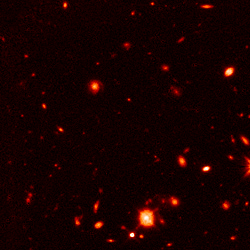
\includegraphics[width=4.0cm]{images/frame_clean.png}}
%  \vspace{1.5cm}
  \centerline{Noiseless frame}\medskip
\end{minipage}
\hfill
\begin{minipage}[b]{0.48\linewidth}
  \centering
  \centerline{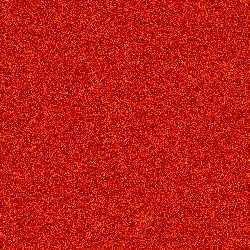
\includegraphics[width=4.0cm]{images/frame.png}}
%  \vspace{1.5cm}
  \centerline{Noisy frame. -30dB SNR}\medskip
\end{minipage}
  \caption{Simulated spacecraft field of view.  False color.}
\label{fig:scene}
\end{figure}

% ------------------- Algorithm ----------------------
\section{Observation Model and Algorithm}
\label{sec:algorithm}

Let $\bm{y}_1, ..., \bm{y}_K \in \mathbb{R}^{N_1 \times N_2}$ be an ordered sequence of $K$ noisy observed frames captured at a constant frame rate with constant drift between frames of $\bm{c}=[c_1, c_2]^T$ pixels.

For each $\bm{y}_k$, we have

\begin{equation}
\bm{y}_k = T_{k\bm{c}}(\bm{\mu}) + \bm{n}_k
\label{eq:model}
\end{equation}


where $T_{k\bm{c}}$ is a translation operator by vector $k\bm{c}$ pixels, $\bm{\mu} \in \mathbb{R}^{N_1 \times N_2}$ is a Nyquist sampled version of the ground truth scene (also known as the reference image), and $\bm{n}_k$ is measurement noise.  We have assumed $T_{k\bm{c}}$ to be a circular translation for ease of derivation, which holds approximately true for small $\bm{c}$ relative to the size of a frame.

Note that we have assumed the blurring induced by motion and the imaging system is spatially and temporally invariant.  Since $T_{k\bm{c}}$ is a linear operator, this constant PSF may be incorporated into $\bm{\mu}$ and accounted for after registration.

The solution for the maximum likelihood solution is given by

\begin{equation}
\hat{\bm{c}} = \arg \max_{\bm{c}} \sum_{m=1}^{K-1}\sum_{k=1}^{K-m} (\bm{y}_k \lstar \bm{y}_{k+m})[m\bm{c}]
\label{eq:algorithm_orig}
\end{equation}

which consists of a series of correlations, two summations, and a downsampling by $m$.  Taking $\arg \max$ over the resultant surface yields the maximum likelihood estimate of the motion, $\hat{\bm{c}}$.

The algorithm can be accelerated by performing correlations in the frequency domain and precomputing the image Fourier transforms with the fast Fourier transform (FFT):

\begin{equation}
\hat{\bm{c}} = \arg \max_{\bm{c}} \sum_{m=1}^{K-1} D_m \left[
\mathcal{F}^{-1} \left( \sum_{k=1}^{K-m} \bm{Y}_k \odot \bm{Y}_{k+m} \right)
\right][\bm{c}]
\label{eq:algorithm}
\end{equation}

where $D_m$ is a downsample operator by $m$ pixels (with zero padding to maintain shape), $\mathcal{F}^{-1}$ is the inverse FFT, $\bm{Y}_k$ is the Fourier transform of $\bm{y}_k$, and $\odot$ is the elementwise product operator.
The algorithm can be broken into four steps, shown below and illustrated graphically in Fig. \ref{fig:algorithm}:

\begin{enumerate}
  \item Precompute image Fourier transforms:
    $$\bm{Y}_k=\mathcal{F}(\bm{y}_k) \text{ for } k=1,...,K$$
  \item Compute image correlations and sum into groups by degree of separation $m$:
    $$\bm{S}_m = \mathcal{F}^{-1} \left( \sum_{k=1}^{K-m} \bm{Y}_k \odot \bm{Y}_{k+m} \right) \text{ for } m=1, ..., K-1$$
  \item Downsample correlation groups by degree of separation and sum:
    $$\sum_{m=1}^{K-1} D_m \left[ \bm{S}_m \right]$$
  \item Take the argmax of the resultant surface to find the estimate $\hat{\bm{c}}$
    $$\hat{c} = \arg \max_c \sum_{m=1}^{K-1} D_m \left[ \bm{S}_m \right]$$
\end{enumerate}

\begin{figure}[htb]
  \begin{minipage}[b]{1\linewidth}
    \centering
    \centerline{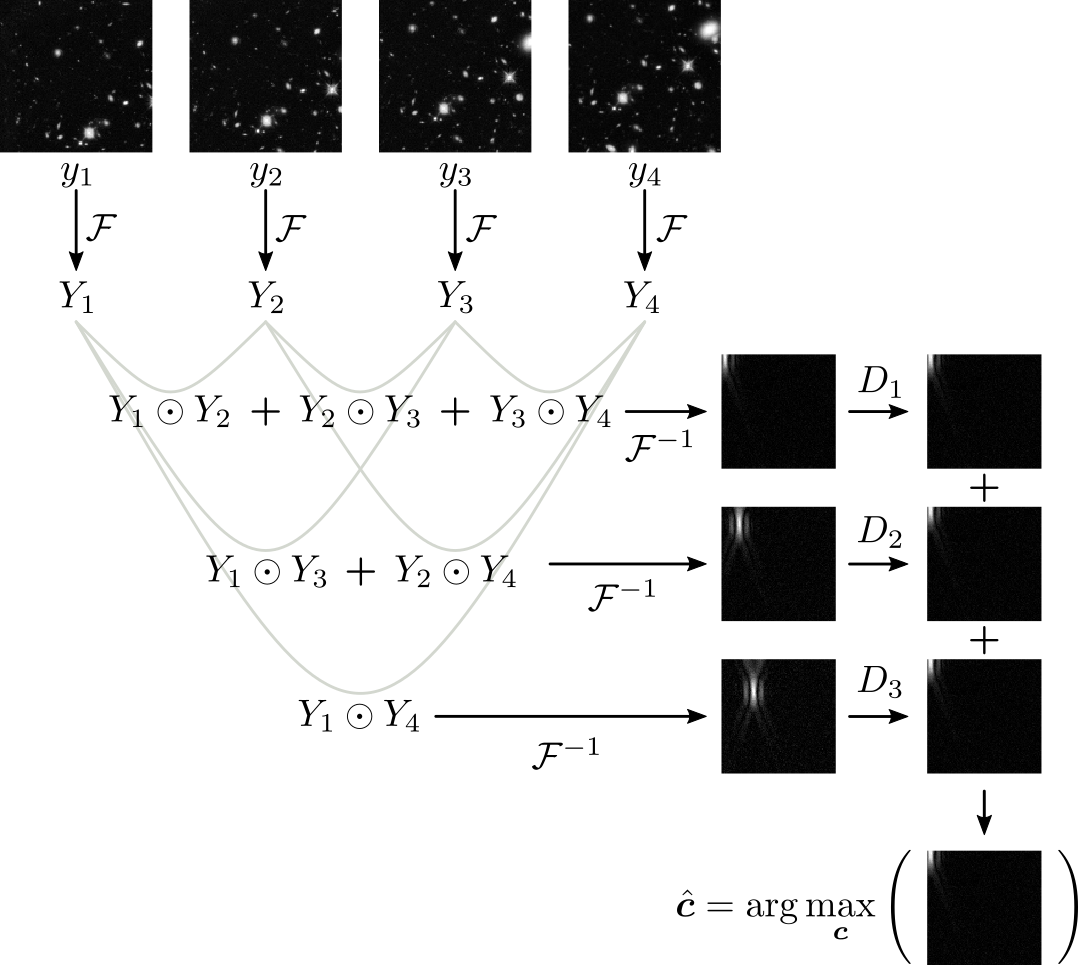
\includegraphics[width=8.5cm]{images/algorithm.png}}
  \end{minipage}
  \caption{Graphical diagram of algorithm given in Equation \ref{eq:algorithm} for a sequence of 4 frames}
  \label{fig:algorithm}
\end{figure}

% ------------------- Optimality ----------------------
\section{Proof of ML Optimality}
\label{sec:optimality}

The proof of optimality is presented in 3 parts:

\begin{enumerate}
\item Derive the expression for likelihood maximization over $\bm{c}$ and $\bm{\mu}$
\item Derive the most likely value for $\mu$ as a function of $c$
\item Show that the log-likelihood solution consists of a sum of downsampled cross correlations
\end{enumerate}

Without loss of generality, we assume the observed frames to be one dimensional vectors of length $N$ and that $c$ is a scalar.

Given the previous observation model

\begin{equation}
y_k = T_{kc}(\mu) + n_k
\end{equation}

assume $n_k \sim \mathcal{N}(0, \sigma^2)$ is additive white Gaussian noise with variance $\sigma^2$.

%***(FIXME: summation offset)

The log-likelihood of having a particular $c$ and $\mu$ given an observation sequence is

\begin{align}
  \hat{c}, \hat{\mu} &= \arg \max_{c, \mu} \ln \mathcal{L}(c, \mu \lpipe y_1, ..., y_K) = \ln \prod_{k=1}^K \mathcal{L}(c, \mu \lpipe y_k) \nonumber \\
  &=\arg \max_{c, \mu} \ln \prod_{k=1}^K \prod_{n=1}^N \mathcal{L}(c, \mu \lpipe y_{k,n}) \nonumber \\
  &=\arg \max_{c, \mu} \ln \prod_{k=1}^K \prod_{n=1}^N \tfrac{1}{\sigma^2 \sqrt{2 \pi}} \text{exp} \left[- \frac{(y_{k,n} - T_{kc}(\mu)_n)^2}{2\sigma^2}\right] \nonumber \\
  &=\arg \min_{c, \mu} \underbrace{\sum_{k=1}^K \sum_{n=1}^N (y_{k,n} - T_{kc}(\mu)_n)^2}_{\text{cost}(c, \mu)} \label{eq:min}
\end{align}

We will take the derivative of the expression denoted cost($c$, $\mu$) in Equation \ref{eq:min} with respect to the $j$th element of $\mu$ to eliminate minimization over $\mu$.

% Due to the circular nature of $T$, some modular arithmetic is necessary, denoted by operator $\%$.

\begin{align}
  &\frac{d}{d\mu_j}\left[\text{cost}(c, \mu)\right] = 0 \nonumber \\
  &=\frac{d}{d\mu_j}\left[\sum_{k=1}^K \sum_{n=1}^N (y_{k,n} - T_{kc}(\mu)_n)^2\right] = 0 \nonumber  \\
  %&=\sum_{k=1}^K \sum_{n=1}^N \frac{d}{d\mu_j}\left[(y_{k,n} - \mu_{kc + n \% N})^2\right] = 0 \nonumber  \\
  %&=\sum_{k=1}^K -2(y_{k,j - kc \% N} - \mu_j)^2 = 0 \nonumber  \\
  %&=\sum_{k=1}^K -2(T_{-kc}(y_k)_j - \mu_j)^2 = 0 \nonumber  \\
  %&=\sum_{k=1}^K -2(T_{-kc}(y_k)_j - \mu_j) = 0 \nonumber  \\
  &\Longrightarrow \hat{\mu}_j = \sum_{k=1}^K T_{-kc}(y_k)_j \nonumber  \\
  &\Longrightarrow \hat{\mu} = \sum_{k=1}^K T_{-kc}(y_k) \label{eq:mu}
\end{align}

This is simply the sum of the motion corrected noisy frames.  Plugging this into the cost function, we obtain an expression that depends only on $c$.  Expanding and eliminating constant terms, we get


\begin{align*}
  &\text{cost}(c, \hat{\mu}) = \text{cost}(c) \\
  &=\sum_{k=1}^K \sum_{n=1}^N \left(y_{k,n} - T_{kc}\left(\sum_{l=1}^K T_{-lc}(y_l)\right)_n\right)^2 \\
  &=\sum_{k=1}^K \sum_{n=1}^N \cancel{y_{k,n}^2} -2y_{k,n}\sum_{l=1}^K T_{(k-l)c}(y_l)_n + \left[\sum_{l=1}^K T_{(k-l)c}(y_l)_n\right]^2 \\
  &=\sum_{\substack{k=1 \\ l=1}}^K \sum_{n=1}^N -2y_{k,n} T_{(k-l)c}(y_l)_n +
  \sum_{k=1}^K \sum_{n=1}^N \left[\sum_{l=1}^K T_{(k-l)c}(y_l)_n\right]^2 \\
\end{align*}

Examining the first term in the cost function, we see it is simply a downsampled correlation between $y_k$ and $y_l$:

$$\sum_{\substack{k=1 \\ l=1}}^K \sum_{n=1}^N -2y_{k,n} T_{(k-1)c}(y_l)_n = -2\sum_{\substack{k=1 \\ l=1}}^K (y_k \lstar y_l) [(k-l)c]$$

Similarly, the second term can be manipulated into a cross correlation:

\begin{align*}
  &\sum_{k=1}^K \sum_{n=1}^N \left[\sum_{l=1}^K T_{(k-l)c}(y_l)_n\right]^2 \\
  &= \sum_{k=1}^K \sum_{n=1}^N \left[\sum_{l=1}^K \left( T_{(k-l)c}(y_l)_n \sum_{m=1}^K T_{(k-m)c}(y_m)_n \right)\right] \\
  &= \sum_{k=1}^K \sum_{n=1}^N \sum_{l=1}^K \sum_{m=1}^K T_{(k-l)c}(y_l)_n T_{(k-m)c}(y_m)_n \\
  &= K \sum_{k=1}^K \sum_{l=1}^K (y_k \lstar y_l)[(k-l)c]
\end{align*}

Now we have

\begin{align*}
  \hat{c} &= \arg \min_c \text{cost}(c) \\
  &= \arg \max_c (K - 2) \sum_{k=1}^K \sum_{l=1}^K (y_k \lstar y_l)[(k - l)c] \\
  &= \arg \max_c \sum_{m=1}^{K-1} \sum_{k=1}^{K-m} (y_k \lstar y_{k+m})[mc]
\end{align*}

which is identical to Equation \ref{eq:algorithm_orig} given in the previous section.

% ------------------- Experimental Results ----------------------
\section{Experimental Results}
\label{sec:results}

To evaluate performance of the algorithm, we simulated a series of simulated noisy frames from an astronomical scene (shown in Fig. \ref{fig:recon}a) according to the motion and noise model given in Equation \ref{eq:model}.  We applied our algorithm given in Equation \ref{eq:algorithm} to find an estimate for the motion, and then corrected the noisy frames and coadded them as in Equation \ref{eq:mu} to obtain the reconstruction in Fig. \ref{fig:recon}b.

We repeated this experiment for various noise levels and number of frames.  As shown in Fig. \ref{fig:db_sweep} and corroborated in \cite{gratadour2005sub}, the registration error decreases with number of frames $K$ and is able to obtain less than 1 pixel of mean absolute registration error at -25dB measurement noise for $K=20$ frames, and the same at -30dB for $K=40$.

Next, we compared registration performance against another area-based registration method for astronomical data given in \cite{ginsburg2013bolocam} which is statistically similar to \cite{gratadour2005sub}, originally used for registering images of cosmic dust in infrared.  Since this algorithm has a more general motion model, we project its estimate to the nearest constant, rigid motion estimate.

Fig. \ref{fig:method_compare} shows that our algorithm is able to successfully register images at more than 10dB lower SNR.

\begin{figure}[htb]
\begin{minipage}[b]{.48\linewidth}
  \centering
  \centerline{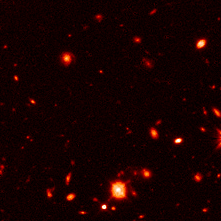
\includegraphics[width=4.0cm]{images/recon_clean.png}}
%  \vspace{1.5cm}
  \centerline{(a) Ground truth}\medskip
\end{minipage}
\hfill
\begin{minipage}[b]{0.48\linewidth}
  \centering
  \centerline{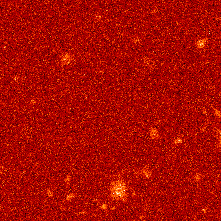
\includegraphics[width=4.0cm]{images/recon.png}}
%  \vspace{1.5cm}
  \centerline{Reconstruction}\medskip
\end{minipage}
  \caption{(b) Reconstruction result for -25dB SNR AWGN and $K=30$ frames.}
\label{fig:recon}
\end{figure}

\begin{figure}[htb]
  \begin{minipage}[b]{1\linewidth}
    \centering
    \centerline{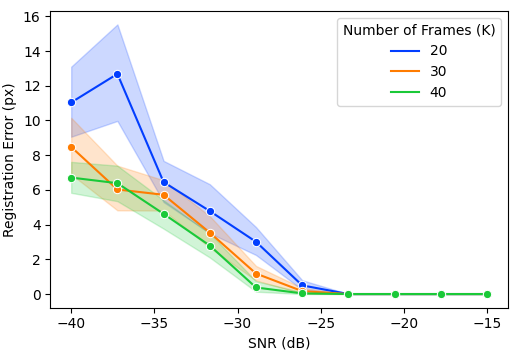
\includegraphics[width=8.5cm]{images/db_sweep.png}}
  \end{minipage}
  \caption{Registration absolute error for various AWGN SNRs and number of frames $K$ with a randomly chosen constant motion vector.}
  \label{fig:db_sweep}
\end{figure}

\begin{figure}[htb]
  \begin{minipage}[b]{1\linewidth}
    \centering
    \centerline{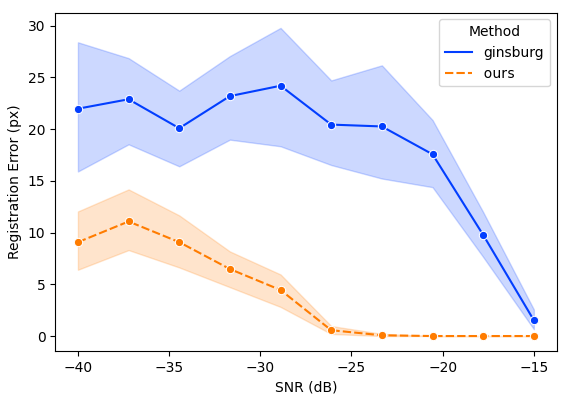
\includegraphics[width=8.5cm]{images/method_compare.png}}
  \end{minipage}
  \caption{Comparison of registration error of our method vs the one presented in \cite{ginsburg2013bolocam} for various noise levels, $K=20$.}
  \label{fig:method_compare}
\end{figure}

% ------------------- Experimental Results ----------------------
\section{Relation to Prior Work}
\label{sec:prior}

In comparison to previous work, our method focuses on the closed form expression of the cost function.  In \cite{gratadour2005sub} and \cite{guillaume1998maximum}, the cost function was not closed form due to the more general motion model which had to be minimized using iterative methods like conjugate gradient descent, requiring evaluation of derivative of the cost.

In contrast, the algorithm here requires only downscaling, multiplication, addition, and FFT methods, which are easily implementable on embedded image processing architectures like an FPGA \cite{bailey2019image}, or are otherwise available as an off-the-shelf IP core \cite{xilinx}.  Additionally, the algorithm is an exhaustive search over the space of all possible motion vectors, requiring no assumptions about the shape of the correlation surface to obtain optimality.

Our method is flexible and can be extended to a subpixel algorithm using the techniques developed in \cite{guizar2008efficient} and \cite{gratadour2005sub}.

% ------------------- Conclusion ----------------------
\section{Conclusion}
\label{sec:future}

In this manuscript, we presented a multiframe registration algorithm for constant rigid motion.  We showed that the algorithm can be realized without iterative maximization methods or parameter tuning, and that under AWGN the algorithm is optimal in the maximum likelihood sense.  Finally, we characterized the algorithm for various noise levels and image sequence lengths and showed our method can obtain accurate registration at 10dB lower than other low SNR registration methods.

\vfill\pagebreak

% References should be produced using the bibtex program from suitable
% BiBTeX files (here: strings, refs, manuals). The IEEEbib.bst bibliography
% style file from IEEE produces unsorted bibliography list.
% -------------------------------------------------------------------------
\bibliographystyle{IEEEbib}
\bibliography{refs}

\end{document}
